\documentclass[11pt]{article}

\marginparwidth 0.5in 
\oddsidemargin 0.25in 
\evensidemargin 0.25in 
\marginparsep 0.25in
\topmargin 0.25in 
\textwidth=6in
\textheight=8in

\usepackage{indentfirst}
\usepackage{graphicx}
\usepackage{caption}
\usepackage{subcaption}

\begin{document}
\hfill\vbox{\hbox{Jude Shin}
		\hbox{CSC 4710-S01}	
		\hbox{Final Project Proposal}	
		\hbox{\today}}\par

\bigskip
\centerline{\Large\bf Maze Exploration}\par
\bigskip

\section{Overview}

I have always been a fan of mazes.
I wrote my first maze generation algorithm in java, so I thought this could be a fun way to showcase it in 3D.
The idea is for a character to explore the maze and try to find the end (treasure or whatnot).
The catch is that there is limited visibility.
The player would have {\tt n} number of lamps that they could pick up and place throughout the maze.
Through those placements, the player would be able to discover different parts of the maze.

Since this is not an algorithms class, I will probably just use a simple recursive backtracker algorithm to generate the maze, although other algorithms might give better visual appeal.

I think making everything dark can be a challenging game mechanic, so I am thinking that the player can toggle between birds eye view (a simple top down approach), or walk the game in first person.

To satisfy the hierarchical transformations, I am going to have a dummy in front of the camera at all times.
When the player is in fps mode, then they will see the dummy running around.
When the player is in birds eye view mode, they will see a tiny dummy running around down there.

Hopefully collision detection will work for the walls, but if the performance takes a big hit, then I might have to implement some regional caching or something. I haven't really thought that far ahead yet.

\section{Concept Art}

Here is an idea of the top down (birds eye) view and fps view that I am considering.

\begin{figure}[h!]
	\centering
	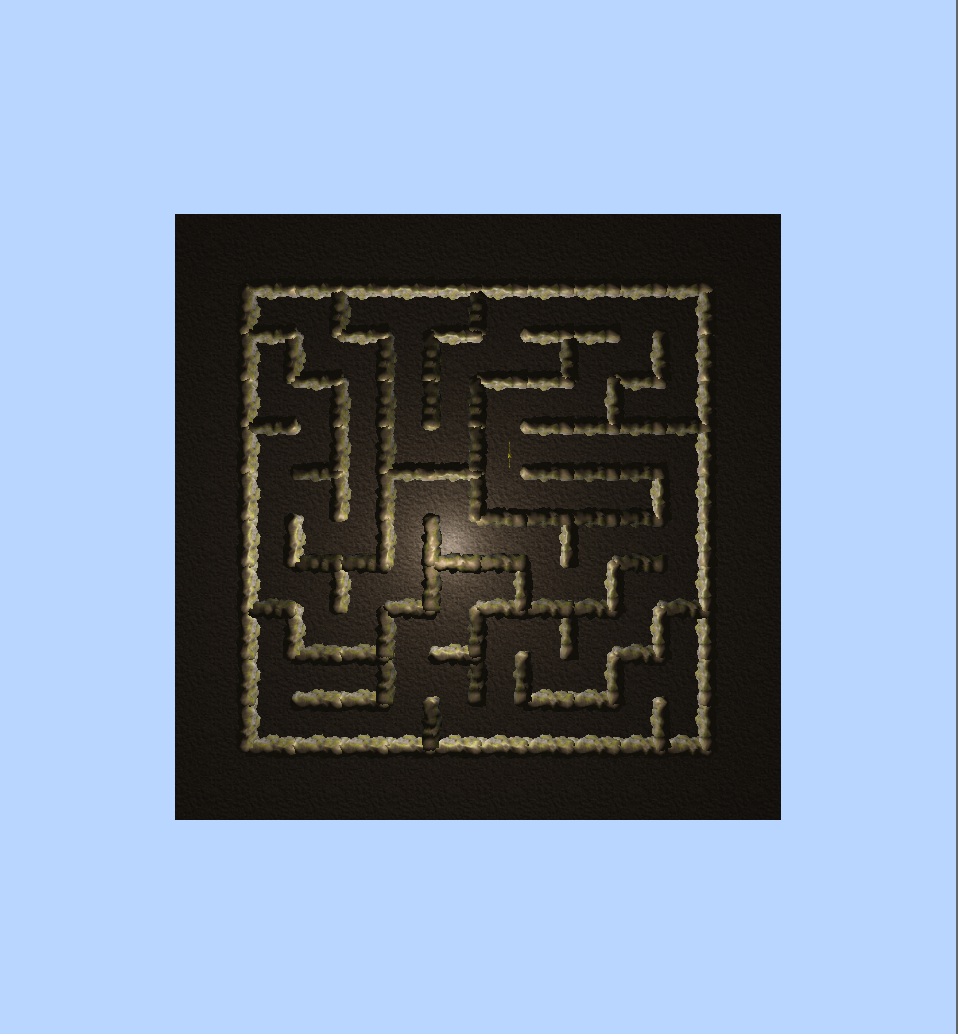
\includegraphics[width=0.9\textwidth]{assets/bird.png}
	\caption{Birds Eye View}
	\label{fig:bird}
\end{figure}

\begin{figure}[h!]
	\centering
	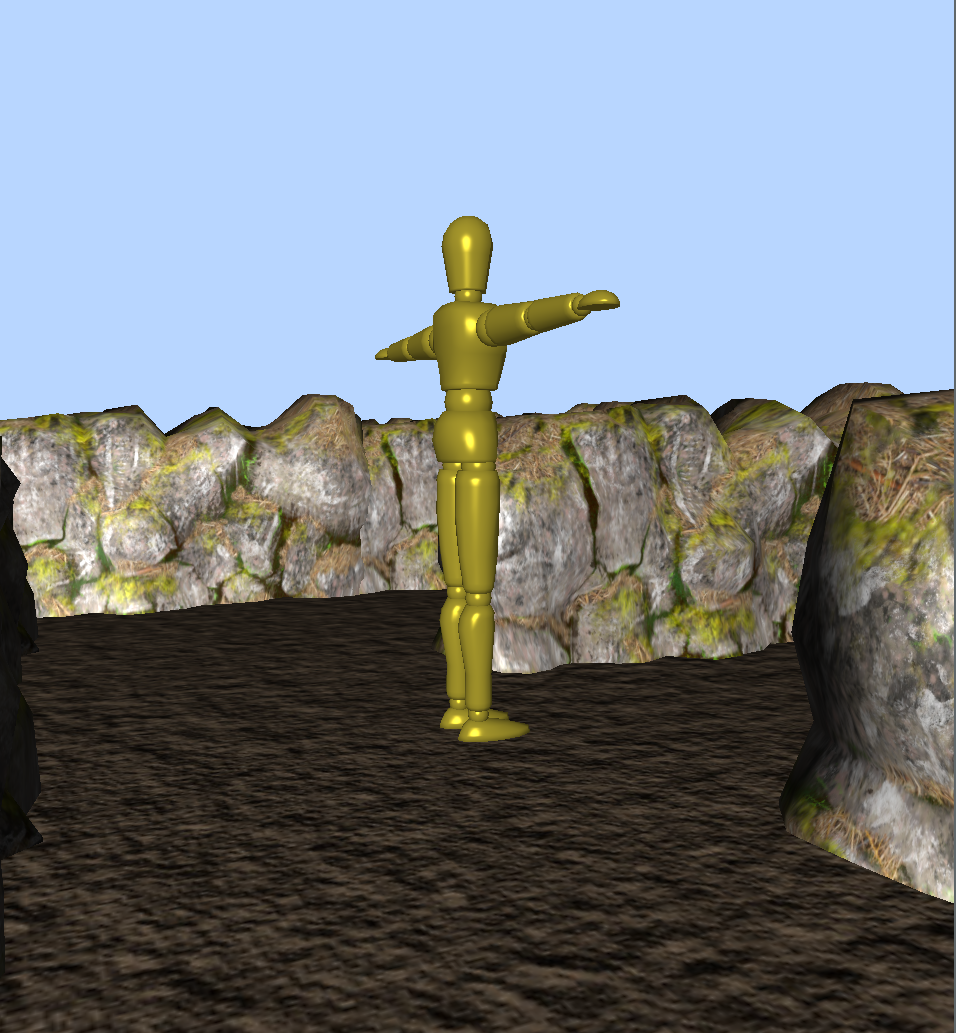
\includegraphics[width=0.9\textwidth]{assets/fps.png}
	\caption{FPS View}
	\label{fig:fps}
\end{figure}

\end{document}
